\section{Results}
\label{sec:results}

Table~\ref{tab:main-results} gives the main comparison, one row per reference class and, for the Monte Carlo reference, one row per variant of the exposure case; the subsections that follow read it by class, and Table~\ref{tab:outcomes} closes the section with the outcome on each hypothesis.

\begin{table}[htbp]
\centering
\small
\caption{Main comparison: every reference class against the engine, with the number compared, the result with its size, and the outcome of the rule fixed for the class; $z$ is the standardised difference of ORE and the engine on the product's draws, and the three collateralised rows are the reported gaps.}
\label{tab:main-results}
\begin{tabular}{p{3.9cm}p{3.2cm}p{5.6cm}l}
\toprule
Reference (class) & Compared & Result & Outcome \\
\midrule
Printed answers, five papers (P) & 438 printed numbers & 313 agree to the digit; 125 gaps listed, largest 35.8 units & gaps explained in part \\
Independent routes (I) & \relax 72 $p$-values, grid of 36 & \relax largest difference $5.7\times10^{-12}$, tolerance $10^{-9}$ & agree \\
Independent routes (I) & \relax 1200 $p$-values, seeded draw & \relax largest difference $8.3\times10^{-12}$ & agree \\
Closed forms in QuantLib (F) & 4 cases of the product & \relax largest relative difference $9.5\times10^{-8}$, gate $10^{-6}$ & agree \\
Closed forms in QuantLib (F) & 297 seeded cases & \relax 296 within the gate; largest $1.6\times10^{-6}$ & one case beyond \\
\relax Cohort estimators in \texttt{transitionMatrix} (F) & 7,350 matrix elements, 30 panels & \relax largest difference $2.2\times10^{-16}$ & agree, two findings \\
Appendix of Hull and White 2012 (P) & 9 printed numbers & 8 agree to the digit; one at 1.32 units & agree within two units \\
Exposure of the single swap (M) & 33 dates, EEPE, CVA & \relax 0 dates beyond 2; largest $\lvert z\rvert$ 0.78; EEPE $z$ +0.30, CVA $z$ +0.37 & agree \\
Exposure of the netting set (M) & 33 dates, EEPE, CVA & \relax 0 dates beyond 2; largest $\lvert z\rvert$ 0.72; EEPE $z$ +0.31, CVA $z$ +0.40 & agree \\
Exposure under a CSA, 10 days (M) & 33 dates, EEPE, CVA & \relax 16 dates beyond 2; largest $\lvert z\rvert$ 9.93; EEPE $z$ -1.55, CVA $z$ -15.89 & gap \\
Exposure under a CSA, 20 days (M) & 33 dates, EEPE, CVA & \relax 12 dates beyond 2; largest $\lvert z\rvert$ 7.09; EEPE $z$ -2.20, CVA $z$ -9.88 & gap \\
Exposure under a CSA with initial margin (M) & 33 dates, EEPE, CVA & \relax 1 dates beyond 2; largest $\lvert z\rvert$ 11.74; EEPE $z$ -0.71, CVA $z$ -1.40 & gap \\
\bottomrule
\end{tabular}
\end{table}


\subsection{Printed answers}
\label{sec:results-printed}

Of the \nPrintedN\ printed numbers of the five papers, \nPrintedAgree\ (\nPrintedShare\,\%) agree with the engine to the printed digit, \nPrintedRecAgree\ of the \nPrintedRecN\ that are recomputed from the committed inputs and \nPrintedReadAgree\ of the \nPrintedReadN\ that are read as the committed documents record them (Table~\ref{tab:printed}). The \nMissTotal\ numbers that miss are not scattered: Figure~\ref{fig:printed-gaps} shows each source with the size of its gaps in units of the last printed digit. The largest gaps among the recomputed cells are in Tasche's Table 9 (\nTableNineMaxUnits\ units), his Table 6 (\nTableSixMaxUnits) and Pluto and Tasche's Table 12 (\nTwelveMaxUnits); the multi-period Tables 13 and 14 of Pluto and Tasche have \nTfourteenAgree\ of \nTfourteenN\ cells within the digit rule, and Schuermann and Hanson's \nSHN\ numbers all agree. By the size of the gap, \nBinHalf\ numbers are within half a unit, \nBinOne\ more within one unit, \nBinTwo\ more within two, and \nBinBeyond\ lie beyond two units. Relaxing the digit rule to one, two and five units raises the agreeing count to \nAgreeOneUnit, \nAgreeTwoUnits\ and \nAgreeFiveUnits, which shows how much of the disagreement is the rounding convention and how much is a different computation.

\begin{table}[htbp]
\centering
\small
\caption{Printed numbers of five papers recomputed with the engine or read as the committed documents record them, with the count that agrees to the printed digit and the largest absolute gap in units of the last printed digit; the sources of the last three rows keep their inputs outside the repository.}
\label{tab:printed}
\begin{tabular}{p{5.2cm}lrrrr}
\toprule
Source & Inputs & Printed numbers & Agree to the digit & Share (\%) & Largest gap (units) \\
\midrule
Pluto and Tasche 2005, Tables 1 to 12 & recomputed & 168 & 125 & 74 & 9.51 \\
Tasche 2013, Table 5 & recomputed & 17 & 15 & 88 & 1.31 \\
Tasche 2013, Table 6 & recomputed & 17 & 8 & 47 & 12.57 \\
Tasche 2013, Table 9, 2009 & recomputed & 17 & 10 & 59 & 35.79 \\
Tasche 2013, Table 7, 2010 & recomputed & 68 & 54 & 79 & 4.75 \\
Tasche 2013, Table 8, 2010 & recomputed & 4 & 4 & 100 & 0.35 \\
Tasche 2013, Table 7, 2011 & recomputed & 68 & 52 & 76 & 4.20 \\
Tasche 2013, Table 8, 2011 & recomputed & 4 & 3 & 75 & 0.57 \\
Schuermann and Hanson 2004, Table 5 & recomputed & 18 & 18 & 100 & 0.45 \\
Israel et al. 2001, L1 distances & as recorded & 9 & 8 & 89 & 4.23 \\
Engelmann 2024, TTC portfolio and PDs & as recorded & 12 & 12 & 100 & 0.50 \\
Pluto and Tasche 2005, Tables 13 and 14 & as recorded & 36 & 4 & 11 & 5.12 \\
All sources &  & 438 & 313 & 71 & 35.79 \\
\bottomrule
\end{tabular}
\end{table}


\begin{figure}[htbp]
\centering
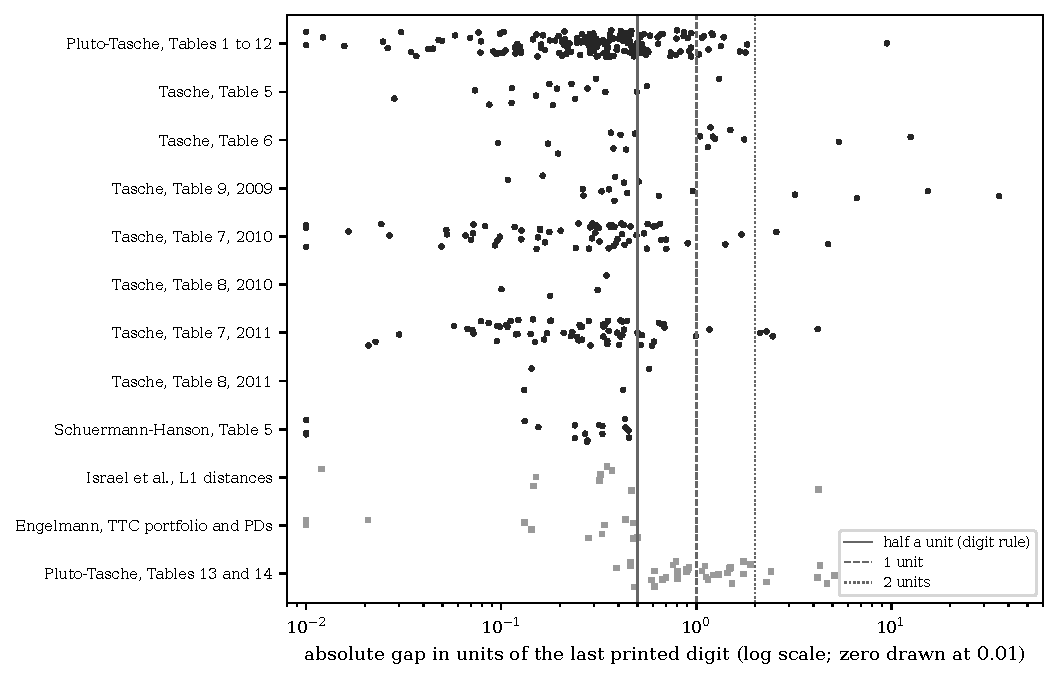
\includegraphics[width=0.96\textwidth]{printed-gaps}
\caption{Absolute gap between the engine and each printed number, in units of the last printed digit and on a logarithmic axis, for each of the twelve source groups; filled circles are recomputed here, squares are read as the committed documents record them, and the vertical lines mark the digit rule of half a unit, one unit and two units.}
\label{fig:printed-gaps}
\end{figure}

The design document quotes \nSddN\ printed numbers and \nSddAgree\ agreeing. Those two counts are reproduced exactly, \nWithoutN\ and \nWithoutAgree, when the three groups of Tasche's Tables 8 and 9 (the case-3 forecasts of 2010 and 2011 and the 2009 likelihood ratios) are left out of the tally; with them the count is \nPrintedN\ and \nPrintedAgree, the one the product's notebook prints. The first hypothesis is therefore not met as stated, because its counts differ from the full tally; the recomputation of which numbers it counts is the contribution of this paragraph. That the two counts come out when those tables are left out is a numerical reconstruction: it does not show that the design document left them out, and no other subset was searched. The choice between the two tallies belongs to the design document.

The explanation of the gaps (Table~\ref{tab:miss-categories}) is a mixture. A rounding explanation is tested here for the scaled bounds: Pluto and Tasche scale the bounds of their Tables 4 and 8, which they print rounded, and scaling the printed bounds in place of the exact ones raises the agreeing cells of Tables 9 to 12 from \nScaledExact\ to \nScaledPrinted\ of \nScaledN\ (Table~\ref{tab:explain-scaled}); the remaining \nScaledLeft\ cells are not explained by rounding. The one miss of Table 4 at a confidence level of $75\,\%$ is explained by the level of the print: the exact bound is $\nFourAtSeventyFive\,\%$ at $0.75$ and $\nFourAtSeventySixThree\,\%$ at $0.763$, and every level from $\nFourLevelLow$ to $\nFourLevelHigh$ prints as the paper's $0.65$. Beyond these \nMissTested\ tested explanations, \nMissRecorded\ gaps carry an explanation recorded in the committed documents and not retested here (\nMissTol\ within a tolerance the engine documents for the table, \nMissAbove\ cells of Table 8 printed at or above the exact bound, \nMissMC\ Monte Carlo prints of Tables 13 and 14, and the one printed generator), and \nMissNone\ have none: \nMissNoneIn\ within one unit and \nMissNoneOut\ beyond it.

\begin{table}[htbp]
\centering
\small
\caption{The scaled bounds of Tables 9 to 12 of Pluto and Tasche, computed from the exact bounds and from the printed and rounded bounds of Tables 4 to 8 that the paper scaled, with the count of cells that agree to the printed digit and the worst gap in units of the last digit for each route.}
\label{tab:explain-scaled}
\begin{tabular}{lrrrrr}
\toprule
Table of Pluto and Tasche & Cells & Agree, exact bounds & Agree, printed bounds & Worst gap, exact & Worst gap, printed \\
\midrule
Table 9 & 24 & 23 & 24 & 0.52 & 0.48 \\
Table 10 & 24 & 21 & 24 & 0.74 & 0.50 \\
Table 11 & 24 & 13 & 21 & 1.83 & 1.13 \\
Table 12 & 24 & 12 & 23 & 9.51 & 8.96 \\
\bottomrule
\end{tabular}
\end{table}

\begin{table}[htbp]
\centering
\small
\caption{The gaps of the printed-answer reconciliation by what explains them: a rounding explanation tested here, a recorded tolerance or note of the committed documents, or none, with the count of gaps in each class over the 438 printed numbers.}
\label{tab:miss-categories}
\begin{tabular}{p{9cm}r}
\toprule
Explanation of the gap & Gaps \\
\midrule
rounded printed inputs (tested) & 24 \\
confidence level of the print (tested) & 1 \\
documented tolerance (recorded) & 48 \\
print at or above the exact bound (recorded) & 12 \\
Monte Carlo print (recorded) & 32 \\
printed generator (recorded) & 1 \\
no explanation; within one unit & 4 \\
no explanation; beyond one unit & 3 \\
All gaps & 125 \\
\bottomrule
\end{tabular}
\end{table}


The printed values of the Appendix of Hull and White are the second hypothesis of the printed class. The engine reproduces \nWWAgree\ of the \nWWN\ printed numbers to the digit. The exception is the second calibration constant: the printed $a(t_2^{*})=-7.8509$ against the recomputed $\nWWAtwo$, a gap of \nWWAtwoUnits\ units; a plain bisection written independently of the engine agrees with the engine to $\nWWBisection$ on both constants, so the difference does not come from the root-finding of the engine. The digit rule of the protocol, fixed before the comparison, does not accept this gap, so the hypothesis is not met as stated. The engine's own test accepts the same constant at an absolute tolerance of $\nWWTestTol$, which is two units of the fourth decimal; that tolerance is not a rule of this protocol, and a rule of two units would have been a choice made after this result. Whether the gap belongs to the paper's arithmetic, to its rounding or to the transcription of its printed digits was not isolated: the printed digits are those of the engine's test file, and no open copy of the paper was read.

\subsection{Independent routes and the reuse trap}
\label{sec:results-routes}

On the grid of \nGridCases\ cases, the engine's Jeffreys $p$-values differ from the quadrature of the Beta density by at most $\nGridJeffMax$ and its binomial $p$-values from the exact rational sum by at most $\nGridBinMax$, so all \nGridWithin\ comparisons are within the tolerance of $10^{-9}$ (Figure~\ref{fig:routes}, left). On \nRandomCases\ cases drawn with a fixed seed the largest differences are $\nRandomJeffMax$ and $\nRandomBinMax$ and all \nRandomWithin\ of \nRandomComparisons\ comparisons are within the tolerance. A comparison with the engine's own SciPy call gives a difference of exactly $\nSameCallGap$ on every case, as Proposition~\ref{prop:reuse} requires. The second hypothesis holds.

\begin{figure}[htbp]
\centering
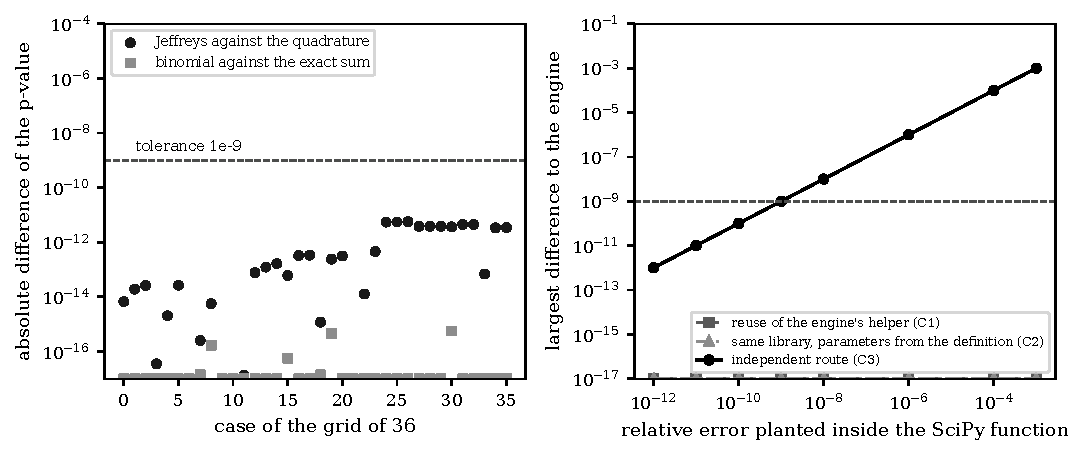
\includegraphics[width=\textwidth]{routes}
\caption{Left: absolute difference between the engine's $p$-values and the two independent routes on the 36 cases of the grid, on a logarithmic axis with the tolerance of $10^{-9}$. Right: largest difference of the defective binomial test to the three kinds of reference as a relative error is planted inside the SciPy function; the reuse and same-library references stay at zero.}
\label{fig:routes}
\end{figure}

Planting defects separates the references (Table~\ref{tab:routes-defects}, Figure~\ref{fig:routes}, right). Moving the tail convention of the binomial helper by one gives a difference of $\nTailGap$ between the defective engine and either the same SciPy function with the parameters written from the definition (C2) or the independent route (C3); the reuse of the engine's helper (C1) gives zero. A relative error planted inside SciPy itself is invisible to C1 and C2 at every size from $10^{-12}$ to $10^{-3}$, whose differences are exactly zero, and the independent route sees it as a difference equal to the planted error: an error of $10^{-9}$ is flagged only at the tolerance itself, because the difference is $\nEpsNineGap$ and exceeds the tolerance by $\nEpsNineExcess$, and errors of $10^{-10}$ and below are not. The independent route is therefore as sharp as its own arithmetic, about $\nGridJeffMax$ for the Jeffreys quadrature, and the library-level defects that a same-library comparison cannot show are the ones it shows.

\begin{table}[htbp]
\centering
\small
\caption{Largest difference between the defective engine's binomial p-value and three kinds of reference on the grid of 36 cases, for a tail convention moved by one and for a relative error planted inside SciPy; a defect is flagged when the difference exceeds the tolerance of $10^{-9}$.}
\label{tab:routes-defects}
\begin{tabular}{p{4.6cm}lllll}
\toprule
Planted defect & Size & C1 reuse & C2 same library & C3 independent & Flagged by \\
\midrule
Tail convention of the binomial helper moved by one & n/a & $0$ & $3.1\times10^{-1}$ & $3.1\times10^{-1}$ & C2 and C3 \\
\relax Relative error $\epsilon$ in SciPy & $1\times10^{-12}$ & $0$ & $0$ & $1.0\times10^{-12}$ & none \\
\relax Relative error $\epsilon$ in SciPy & $1\times10^{-11}$ & $0$ & $0$ & $1.0\times10^{-11}$ & none \\
\relax Relative error $\epsilon$ in SciPy & $1\times10^{-10}$ & $0$ & $0$ & $1.0\times10^{-10}$ & none \\
\relax Relative error $\epsilon$ in SciPy & $1\times10^{-9}$ & $0$ & $0$ & $1.0\times10^{-9}$ & C3 \\
\relax Relative error $\epsilon$ in SciPy & $1\times10^{-8}$ & $0$ & $0$ & $1.0\times10^{-8}$ & C3 \\
\relax Relative error $\epsilon$ in SciPy & $1\times10^{-6}$ & $0$ & $0$ & $1.0\times10^{-6}$ & C3 \\
\relax Relative error $\epsilon$ in SciPy & $1\times10^{-4}$ & $0$ & $0$ & $1.0\times10^{-4}$ & C3 \\
\relax Relative error $\epsilon$ in SciPy & $1\times10^{-3}$ & $0$ & $0$ & $9.9\times10^{-4}$ & C3 \\
\bottomrule
\end{tabular}
\end{table}


\subsection{Closed forms and the transition-matrix library}
\label{sec:results-closed}

The four closed-form cases of the product agree with QuantLib: the bond call and put to the last bit (a relative difference of exactly $0$) and the payer and receiver swaptions to $\nSwaptionPayer$ and $\nSwaptionReceiver$ (Figure~\ref{fig:closed-forms}, left, and Table~\ref{tab:main-results}). On \nClosedCases\ cases of a seeded grid of mean reversion, volatility, expiry, maturity and strike, the median relative difference is $\nClosedMedian$ and \nClosedWithin\ of the cases are within the gate of $10^{-6}$. The one case beyond the gate, a receiver swaption, differs by $\nClosedMax$ relative, which is an absolute difference of $\nClosedWorstAbs$ USD on a price of \nClosedWorstPrice\ USD for a notional of one million: the option is deep out of the money, which makes a relative gate demanding there. The size of the price does not explain the case by itself: a bond call of the same grid, priced at $\nClosedBondPrice$ USD, differs from QuantLib by only $\nClosedBondRel$ relative. The cause, for which QuantLib's root-finding tolerance in the swaption pricer is a candidate, was not isolated. The fourth hypothesis holds on the four cases of the product and fails the relative gate in one of \nClosedCases\ cases of the grid, so it is not met as stated; an absolute floor of the kind that Section~\ref{sec:proposed-closed} proposes would accept the case, but it was added after the result and is not the rule under which the hypothesis was judged.

\begin{figure}[htbp]
\centering
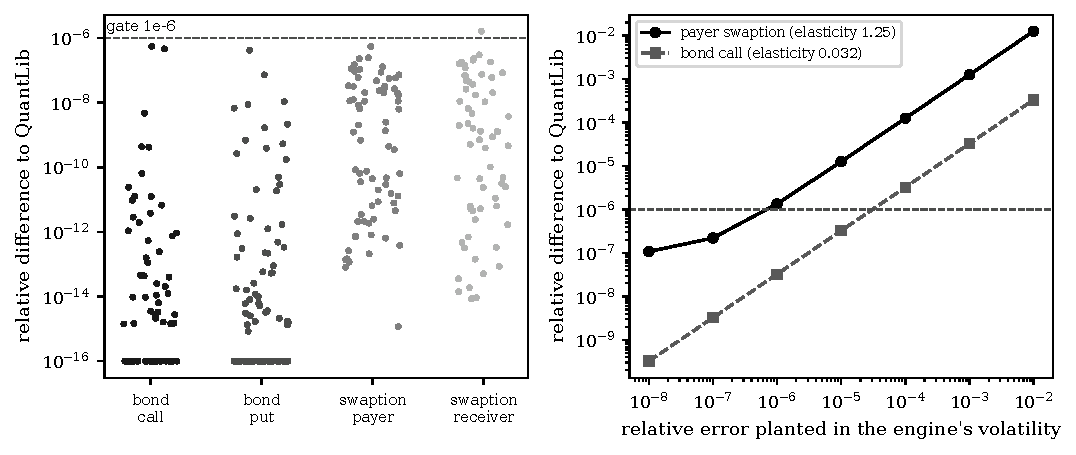
\includegraphics[width=\textwidth]{closed-forms}
\caption{Left: relative difference between the engine's closed forms and QuantLib on the seeded grid, by instrument, on a logarithmic axis with the gate of $10^{-6}$. Right: relative difference to QuantLib as a relative error is planted in the engine's volatility, for a payer swaption of elasticity to volatility near one and for a deep in-the-money bond call of elasticity near $0.03$.}
\label{fig:closed-forms}
\end{figure}

The sensitivity of the gate follows Proposition~\ref{prop:gate}. The measured elasticities to volatility are \nElasticitySwaption\ for the swaption and \nElasticityBond\ for the bond call, so the gate flags a volatility error of $\nDetectSwaption$ in the first and of $\nDetectBond$ in the second; the planted errors confirm it (Figure~\ref{fig:closed-forms}, right): an error of $10^{-6}$ is flagged on the swaption and not on the bond call, whose relative difference is $\nBondAtMillionth$.

The cohort estimators of the engine, compared with \texttt{transitionMatrix} \nTMVersion\ on \nTMPanels\ seeded panels (Table~\ref{tab:transition-matrix}), agree to $\nTMMaxDiff$ over \nTMElements\ matrix elements once the conventions of the package are aligned: the withdrawals kept as a state or excluded, per period or pooled. Two differences remain, and each is explained by the package's code. The package counts the last migration of its last entity twice, which moves its matrix by $\nTMDoubleMin$ to $\nTMDoubleMax$; adding that one migration to the engine's counts reproduces the package's matrix to $\nTMDoubleFixed$. And the package's Aalen--Johansen increment divides by the risk set after the exit, giving $\nTMAJPackage$ where the engine gives $\nTMAJEngine$ on a four-obligor example.

\begin{table}[htbp]
\centering
\small
\caption{The engine's cohort and Aalen--Johansen estimators against \texttt{transitionMatrix} 0.5.1 on 30 seeded panels of 600 entities with withdrawals: the largest element-wise difference for each convention, and the two differences that the package's own code explains.}
\label{tab:transition-matrix}
\begin{tabular}{p{6.3cm}p{2.8cm}p{5.2cm}}
\toprule
Comparison & Largest difference & Outcome \\
\midrule
Cohort, withdrawals kept as a state, per period & $0$ & agree \\
Cohort, withdrawals kept as a state, pooled & $0$ & agree \\
Cohort, withdrawals excluded, per period & $2.2\times10^{-16}$ & agree \\
Cohort, withdrawals excluded, pooled & $2.2\times10^{-16}$ & agree \\
Last record of the last entity, package unguarded & 0.0013 to 0.0016 & gap: the package counts the last migration twice \\
Same, engine counts corrected by that migration & $0$ & explained \\
Aalen--Johansen increment on the four-obligor example & 0.0833 & gap: risk set counted after the exit (3 against 4) \\
\bottomrule
\end{tabular}
\end{table}


\subsection{The Monte Carlo reference on the product's draws}
\label{sec:results-committed}

On the product's draws (seed 42 for both engines), the single swap and the netting set pass the rule: no report date is beyond two combined standard errors, the largest $\lvert z\rvert$ is \nSingleMaxZ\ and \nNettingMaxZ, and the EEPE and CVA differences are \nSingleEepeZ\ and \nSingleCvaZ\ (single swap) and \nNettingEepeZ\ and \nNettingCvaZ\ (netting set) combined standard errors (Table~\ref{tab:committed-ore}, Figure~\ref{fig:z-profiles}). The third hypothesis holds on those draws. The three collateralised variants do not: the 10-day variant has \nCsaTenBeyond\ of 33 dates beyond two, a largest $\lvert z\rvert$ of \nCsaTenMaxZ\ and a CVA difference of \nCsaTenCvaZ\ combined standard errors; the 20-day variant \nCsaTwentyBeyond\ dates, \nCsaTwentyMaxZ\ and \nCsaTwentyCvaZ; and the variant with initial margin \nImBeyond\ date beyond two in the expected exposure, the last report date at 9.5 years, with a $\lvert z\rvert$ of \nImMaxZ, and a mean dynamic initial margin of ORE at \nImRatio\ of the engine's, with all \nImDimBeyond\ dates of the margin beyond two (largest \nImDimMaxZ). These are the gaps the sixth hypothesis lists, and the measured values match its figures of $9.9$, $7.1$ and $11.7$, $15.9$ and $9.9$, and $0.88$.

\begin{table}[htbp]
\centering
\footnotesize
\setlength{\tabcolsep}{4pt}
\caption{The five exposure variants reconciled with ORE on the product's draws. Panel A: the number of the 33 report dates beyond two combined standard errors, the largest and the mean standardised difference, and the EEPE and CVA differences. Panel B: the largest standardised difference of the diagnostic run with a zero minimum transfer amount (MTA), and the equivalence margin and the 80 percent detectable gap of the EEPE.}
\label{tab:committed-ore}
\textbf{A. The differences}\par\smallskip
\begin{tabularx}{\textwidth}{@{}>{\raggedright\arraybackslash}X>{\raggedleft\arraybackslash}p{2.0cm}>{\raggedleft\arraybackslash}p{2.2cm}>{\raggedleft\arraybackslash}p{1.8cm}>{\raggedleft\arraybackslash}p{1.8cm}>{\raggedleft\arraybackslash}p{1.8cm}@{}}
\toprule
Variant & Dates beyond 2 & \relax Largest $\lvert z\rvert$ & \relax Mean $z$ & \relax EEPE $z$ & \relax CVA $z$ \\
\midrule
Single swap & 0 & 0.78 & +0.17 & +0.30 & +0.37 \\
Netting set & 0 & 0.72 & +0.18 & +0.31 & +0.40 \\
CSA, 10 days & 16 & 9.93 & -2.38 & -1.55 & -15.89 \\
CSA, 20 days & 12 & 7.09 & -1.47 & -2.20 & -9.88 \\
CSA, 10 days, initial margin & 1 & 11.74 & -0.19 & -0.71 & -1.40 \\
\bottomrule
\end{tabularx}
\par\medskip
\textbf{B. The diagnostic run and what a pass supports}\par\smallskip
\begin{tabularx}{\textwidth}{@{}>{\raggedright\arraybackslash}X>{\raggedleft\arraybackslash}p{3.0cm}>{\raggedleft\arraybackslash}p{3.4cm}>{\raggedleft\arraybackslash}p{3.4cm}@{}}
\toprule
Variant & \relax Largest $\lvert z\rvert$, zero MTA & EEPE equivalence margin (\%) & EEPE detectable gap (\%) \\
\midrule
Single swap & n/a & 1.9 & 2.8 \\
Netting set & n/a & 2.1 & 3.1 \\
CSA, 10 days & 3.64 & 2.3 & 2.0 \\
CSA, 20 days & 4.17 & 2.7 & 2.0 \\
CSA, 10 days, initial margin & n/a & 23.1 & 27.9 \\
\bottomrule
\end{tabularx}
\end{table}


\begin{figure}[htbp]
\centering
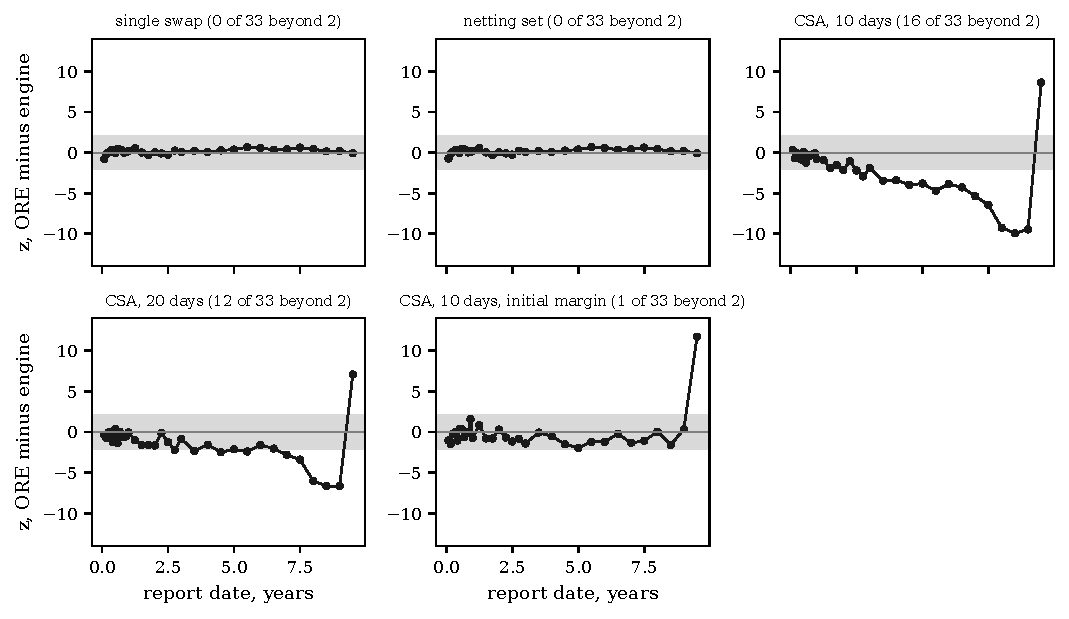
\includegraphics[width=\textwidth]{z-profiles}
\caption{Standardised difference z between ORE and the engine at the 33 report dates for the five exposure variants on the product's draws, with the band of two combined standard errors shaded; the uncollateralised variants stay inside the band, the collateralised ones leave it from two to three years on and again at the last date, and the initial-margin variant leaves it only at the last report date of 9.5 years.}
\label{fig:z-profiles}
\end{figure}

For the collateralised variants the diagnostic run with a zero minimum transfer amount in both engines lowers the largest $\lvert z\rvert$ from \nCsaTenMaxZ\ to \nCsaTenMtaZ\ (10 days) and from \nCsaTwentyMaxZ\ to \nCsaTwentyMtaZ\ (20 days). It does not remove the gap, so the minimum transfer amount explains part of it and the remainder is not explained, which the product's case page also leaves open.

What the passes show is bounded by the standard errors (Table~\ref{tab:committed-ore}, last two columns). The EEPE difference of the single swap supports equivalence within $\nSingleEquivalence\,\%$ of its value at the $5\,\%$ level and the rule detects a systematic gap of $\nSingleDetectable\,\%$ with probability $0.8$; for the netting set the two numbers are $\nNettingEquivalence\,\%$ and $\nNettingDetectable\,\%$. The agreement is an agreement to about two percent of the effective exposure, not an equality.

\subsection{The same comparison on new seeds}
\label{sec:results-seeds}

Rerunning the comparison with ORE on new seeds (Table~\ref{tab:ore-replicates}, Figure~\ref{fig:ore-replicates}) shows whether the product's outcomes are properties of the engines or of the draws. The rule passes on \nReplNetPass\ of \nReplNetN\ seeds for the netting set (Wilson interval \nReplNetLo\ to \nReplNetHi\,\%) and on \nReplSinPass\ of \nReplSinN\ for the single swap (\nReplSinLo\ to \nReplSinHi\,\%); rerunning the product's seed 42 reproduces the committed standardised differences of the four variants to within \nSeedFortyTwoGap\ at every date (largest $\lvert z\rvert$ of \nSeedFortyTwoNetting\ for the netting set against \nNettingMaxZ\ committed). The mean over seeds and dates of $z$ is \nReplNetMeanZ\ and \nReplSinMeanZ\ with the product's errors and \nReplNetMeanZPair\ and \nReplSinMeanZPair\ with the pair-aware ones, so the two engines have no systematic gap larger than a fraction of a combined standard error, in the direction of ORE above the engine. The single swap and the netting set are not two independent results: their replicates use the same seeds and the swap SW-1 is in both books, and from the date at five years on, where the three shorter swaps have matured and both books hold only SW-1, their mean standardised differences are equal to \nSharedMeanGap. The collateralised 10-day variant fails the rule on \nReplCsaFail\ of \nReplCsaN\ seeds, with a mean largest $\lvert z\rvert$ of \nReplCsaMaxZ\ and a mean CVA difference of \nReplCsaCvaZ\ combined standard errors: the gap of the 10-day variant is a property of the two engines, not of the draw. The 20-day and initial-margin variants were run on the product's draws only.

\begin{table*}[htbp]
\centering
\small
\caption{The engine against ORE on new seeds: the number of seeds on which the product's rule passes, the mean standardised difference over seeds and dates with the product's and the pair-aware errors, the mean EEPE and CVA differences, and the largest difference at the product's seed 42 rerun here.}
\label{tab:ore-replicates}
\begin{tabular}{p{3.1cm}rlrrrrrr}
\toprule
Variant & Seeds & Rule passed (95\% interval, \%) & Mean $z$ & Mean $z$, pair-aware & Mean EEPE $z$ & Mean CVA $z$ & Median largest $\lvert z\rvert$ & Largest $\lvert z\rvert$ at seed 42 \\
\midrule
Single swap & 24 & 22 (74--98) & +0.10 & +0.20 & +0.29 & +0.12 & 1.36 & 0.78 \\
Netting set & 24 & 22 (74--98) & +0.10 & +0.20 & +0.29 & +0.12 & 1.38 & 0.72 \\
CSA, 10 days & 8 & 0 (0--32) & -2.18 & -2.90 & -0.12 & -14.57 & 10.82 & 9.93 \\
\bottomrule
\end{tabular}
\end{table*}


\begin{figure}[htbp]
\centering
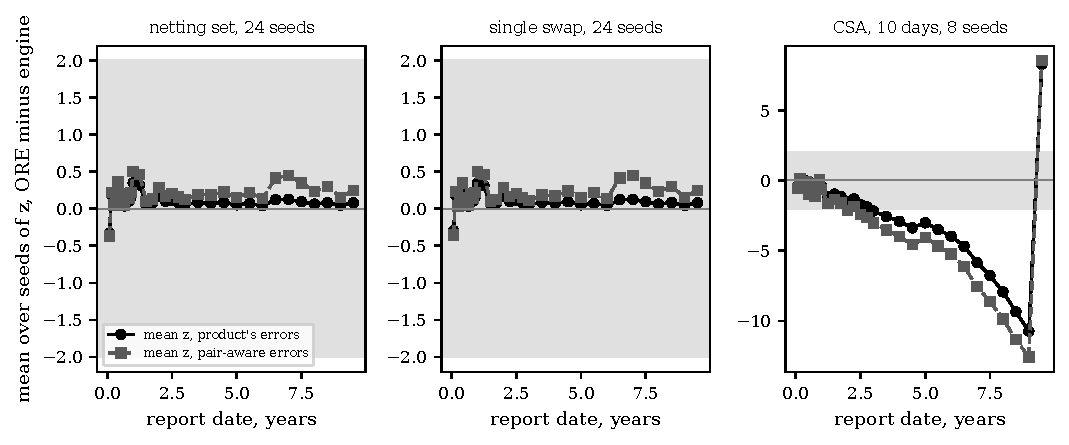
\includegraphics[width=\textwidth]{ore-replicates}
\caption{Mean over the seeds of the standardised difference between ORE and the engine at each report date, for the netting set, the single swap and the 10-day collateralised variant, with the product's standard errors and with pair-aware ones; the shaded band is the acceptance bound of two.}
\label{fig:ore-replicates}
\end{figure}

The predictions written before these runs are reported in Table~\ref{tab:outcomes}, panel B: R1 to R5 are \nPredRone, \nPredRtwo, \nPredRthree, \nPredRfour\ and \nPredRfive. R2 was written after the pilot that had shown the spread of two runs of the engine, so its holding says that the spread transfers to ORE, not that it was foreseen.

\subsection{Calibration of the standard error}
\label{sec:results-calibration}

Two runs of the same model should give a standardised difference of unit variance. They do not when the standard errors treat the paths as independent (Table~\ref{tab:calibration}, Figure~\ref{fig:pairs}). The standard deviation of $z$ over \nCritReps\ paired runs has a median over the report dates of \nSdSingle\ for the single swap and \nSdNetting\ for the netting set, falling from \nSdFirst\ at the first date to \nSdLast\ at the last; for the CVA it is \nSdCvaSingle\ and \nSdCvaNetting. The correlation of the two paths of an antithetic pair is $\nRhoFirst$ at the first date and $\nRhoLast$ at the last, and the spread that Proposition~\ref{prop:antithetic} predicts from it, $\sqrt{1+\rho}$, matches the measured spread at every date with a mean absolute deviation of \nSdDeviation. With pair-aware errors the median spread is \nSdSinglePair\ and \nSdNettingPair. The EEPE, whose error is already a batch error over antithetic blocks, is calibrated: its spread is \nSdEepeSingle\ and \nSdEepeNetting. Figure~\ref{fig:null-z} draws the standardised difference of the product's errors, pooled over the dates, for the first \nNullZReps\ of the \nCritReps\ paired runs (the repetitions that the output stores in full), against the standard normal density: it is narrower, with little mass beyond two, which is why a bound of two applied to one date rejects rarely and why the rule's size comes from the number of comparisons and not from any one of them.

\begin{table}[htbp]
\centering
\footnotesize
\setlength{\tabcolsep}{4pt}
\caption{Standard deviation over 400 paired runs of the same model of the standardised difference, for the product's errors and the pair-aware errors, and for the CVA the value that Proposition~\ref{prop:antithetic} predicts from the measured pair correlation; a calibrated statistic has a standard deviation of one.}
\label{tab:calibration}
\begin{tabularx}{\textwidth}{@{}>{\raggedright\arraybackslash}X>{\centering\arraybackslash}p{2.2cm}>{\centering\arraybackslash}p{2.2cm}>{\centering\arraybackslash}p{2.4cm}>{\centering\arraybackslash}p{2.4cm}@{}}
\toprule
Statistic & Single swap, product errors & Netting set, product errors & Single swap, pair-aware & Netting set, pair-aware \\
\midrule
Expected exposure, dates (median over dates) & 0.62 & 0.62 & 1.00 & 1.00 \\
EEPE (batch error) & 1.03 & 1.03 & n/a & n/a \\
CVA & 0.37 & 0.35 & 0.36 (predicted) & 0.35 (predicted) \\
\bottomrule
\end{tabularx}
\end{table}


\begin{figure}[htbp]
\centering
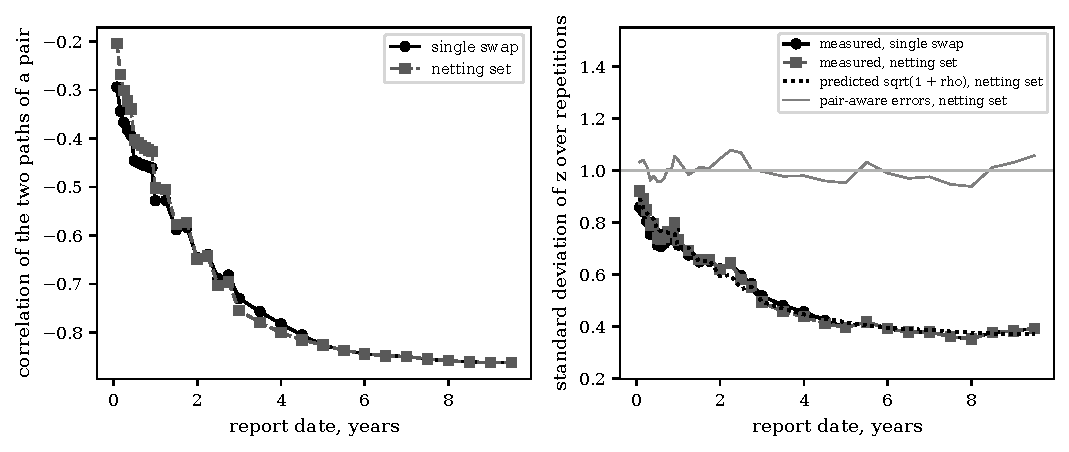
\includegraphics[width=\textwidth]{pairs}
\caption{Left: correlation between the two paths of an antithetic pair of the discounted exposure at each report date, for the single swap and the netting set, averaged over 40 simulations. Right: standard deviation over the paired runs of the standardised difference at each date with the product's errors, with the value $\sqrt{1+\rho}$ predicted from the pair correlation and with pair-aware errors.}
\label{fig:pairs}
\end{figure}

\begin{figure}[htbp]
\centering
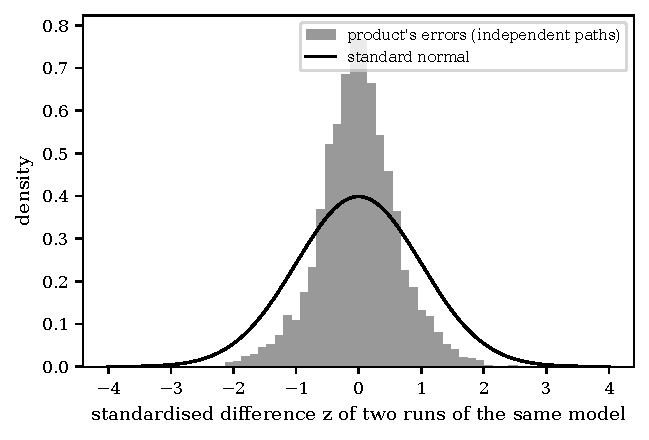
\includegraphics[width=0.62\textwidth]{null-z}
\caption{Histogram of the standardised difference of two runs of the same model on the netting set, pooled over the 33 dates and the first \nNullZReps\ of the \nCritReps\ paired runs, with the product's standard errors, against the standard normal density; the distribution is narrower than the normal because the errors overstate the variance of antithetic means.}
\label{fig:null-z}
\end{figure}

\subsection{Size and power of the acceptance rule}
\label{sec:results-power}

Table~\ref{tab:rule-size-power} and Figure~\ref{fig:power} give the rejection rates of the twelve rules. The product's rule rejects two runs of the same model in \nSizeProdSingle\,\% of the repetitions for the single swap and \nSizeProdNetting\,\% for the netting set, above the nominal $5\,\%$ and well below the $80.4\,\%$ that Proposition~\ref{prop:size} allows for independent comparisons. The rate is the result of two errors of opposite sign: each date's error is overstated, and the family has thirty-five comparisons. Taking the errors alone away, with pair-aware errors and the bound of two, gives a size of \nSizePairNetting\,\%; the bound of $3.18$ with the product's errors gives \nSizeSidakNetting\,\% and a power of \nPowerSidakSigmaTwo\,\% against a $2\,\%$ volatility defect; the two changes together, the refinement of Section~\ref{sec:proposed-refine}, give \nSizeRefineSingle\,\% and \nSizeRefineNetting\,\%, whose intervals contain the nominal size. The intervals of the product's rule, \nSizeProdNettingLo\ to \nSizeProdNettingHi\,\%, do not.

\begin{table*}[htbp]
\centering
\small
\caption{Rejection rate in percent, with its Wilson 95 percent interval, of ten acceptance rules over 400 paired runs of the engine and a reference of the same model: the size on the single swap and on the netting set, and the power on the netting set against a volatility raised by 2 and 5 percent, a mean reversion raised by 50 percent, and a measure error.}
\label{tab:rule-size-power}
\begin{tabular}{p{4.6cm}llllll}
\toprule
Rule & Size, single & Size, netting & Vol. +2 \% & Vol. +5 \% & Rev. +50 \% & Measure \\
\midrule
Product rule (dates, EEPE, CVA; bound 2) & 10.5 [7.9, 13.9] & 12.5 [9.6, 16.1] & 75.0 [70.5, 79.0] & 100.0 [99.0, 100.0] & 100.0 [99.0, 100.0] & 100.0 [99.0, 100.0] \\
Product errors, bound 3.18 & 0.2 [0.0, 1.4] & 0.2 [0.0, 1.4] & 18.5 [15.0, 22.6] & 99.0 [97.5, 99.6] & 100.0 [99.0, 100.0] & 100.0 [99.0, 100.0] \\
Pair-aware errors, bound 2 & 56.0 [51.1, 60.8] & 56.0 [51.1, 60.8] & 99.8 [98.6, 100.0] & 100.0 [99.0, 100.0] & 100.0 [99.0, 100.0] & 100.0 [99.0, 100.0] \\
Pair-aware errors, bound 3.18 & 4.5 [2.9, 7.0] & 3.8 [2.3, 6.1] & 76.5 [72.1, 80.4] & 100.0 [99.0, 100.0] & 100.0 [99.0, 100.0] & 100.0 [99.0, 100.0] \\
Dates only (bound 2) & 6.8 [4.7, 9.6] & 9.5 [7.0, 12.8] & 68.2 [63.5, 72.6] & 100.0 [99.0, 100.0] & 100.0 [99.0, 100.0] & 100.0 [99.0, 100.0] \\
EEPE only (bound 2) & 6.2 [4.3, 9.1] & 6.2 [4.3, 9.1] & 52.5 [47.6, 57.3] & 100.0 [99.0, 100.0] & 100.0 [99.0, 100.0] & 58.5 [53.6, 63.2] \\
CVA only (bound 2) & 0.0 [0.0, 1.0] & 0.0 [0.0, 1.0] & 0.2 [0.0, 1.4] & 100.0 [99.0, 100.0] & 100.0 [99.0, 100.0] & 0.0 [0.0, 1.0] \\
Fixed tolerance 1 \% of the peak & 60.0 [55.1, 64.7] & 30.8 [26.4, 35.4] & 92.5 [89.5, 94.7] & 100.0 [99.0, 100.0] & 100.0 [99.0, 100.0] & 100.0 [99.0, 100.0] \\
Fixed tolerance 2 \% of the peak & 1.0 [0.4, 2.5] & 0.0 [0.0, 1.0] & 10.2 [7.6, 13.6] & 99.5 [98.2, 99.9] & 100.0 [99.0, 100.0] & 100.0 [99.0, 100.0] \\
Fixed tolerance 5 \% of the peak & 0.0 [0.0, 1.0] & 0.0 [0.0, 1.0] & 0.0 [0.0, 1.0] & 0.0 [0.0, 1.0] & 100.0 [99.0, 100.0] & 100.0 [99.0, 100.0] \\
\bottomrule
\end{tabular}
\end{table*}


\begin{figure}[htbp]
\centering
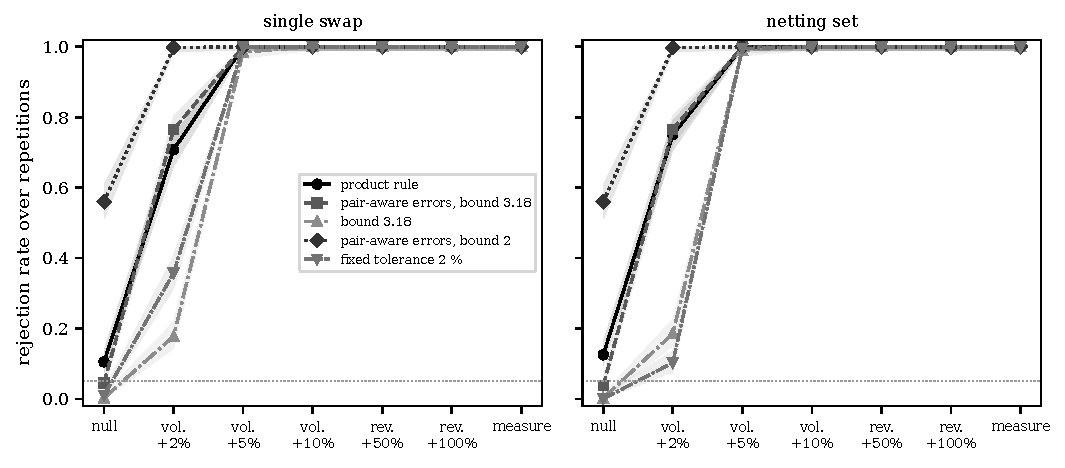
\includegraphics[width=\textwidth]{power}
\caption{Rejection rate of five of the twelve rules over the paired runs under the null and under six planted conditions, for the single swap and the netting set, with the Wilson 95 percent interval shaded; the dotted line marks the nominal size of 5 percent, and the product's rule, the refinement and the pair-aware rule at the bound 2 reject every defect of 5 percent or more, and the fixed tolerance of 2 percent does so on the single swap.}
\label{fig:power}
\end{figure}

The power of the refinement against a volatility raised by $2\,\%$ is \nPowerRefineSigmaTwo\,\% on the netting set, against \nPowerProdSigmaTwo\,\% for the product's rule at a size of \nSizeProdNetting\,\%; at $5\,\%$ both reject in every repetition. A mean reversion raised by half is rejected in every repetition by both. The measure error, which reports the discounted expected exposure where the forward-measure one is meant, is rejected by every rule that reads the profile, and the EEPE alone misses it in \nMeasureEepeMiss\,\% of the repetitions: its error comes from the profile only through the effective maximum, and the CVA, computed from the discounted exposure, is unchanged by it. The fixed tolerances show what the standard error is worth: a tolerance of $1\,\%$ of the peak has a size of \nSizeFixedOneNetting\,\% and one of $2\,\%$ has a power of \nPowerFixedTwoSigmaTwo\,\% against the $2\,\%$ volatility error, where the refinement has \nPowerRefineSigmaTwo\,\%.

The maximum-T comparator answers whether the family-wise bound of $3.18$ gives up power that the dependence of the comparisons would return. Estimated on the other half of the repetitions, the covariance of the 35 differences gives bounds of \nMaxtPairBoundLow\ to \nMaxtPairBoundHigh\ for the pair-aware errors, below the $3.18$ of independent comparisons, and of \nMaxtProdBoundLow\ to \nMaxtProdBoundHigh\ for the product's errors (Table~\ref{tab:rule-size-power}). With pair-aware errors the maximum-T rule has a size of \nSizePairMaxtSingle\,\% on the single swap and \nSizePairMaxtNetting\,\% on the netting set, intervals that contain the nominal $5\,\%$, and a power of \nPowerPairMaxtSigmaTwo\,\% against the $2\,\%$ volatility error on the netting set (\nPowerPairMaxtSigmaTwoLo\ to \nPowerPairMaxtSigmaTwoHi), against \nPowerRefineSigmaTwo\,\% for the bound $3.18$. The two marginal intervals do not overlap, but their overlap is not the test for two rules applied to the same runs. The two rules read the same pair-aware statistic on the same pairs of runs, and the maximum-T bound is the lower one (at most \nMaxtPairBoundHigh\ against $\nSidakBound$), so it rejects in every repetition in which the bound $\nSidakBound$ rejects. It adds \nMaxtExtraNetting\ rejections of \nMaxtPairedReps\ on the netting set under the $2\,\%$ volatility error (\nMaxtGainNetting\ points) and \nMaxtExtraSingle\ on the single swap (\nMaxtGainSingle\ points), and loses none (\nMaxtLostMax). The exact two-sided sign test on the repetitions in which the two rules differ, computed by \texttt{experiments/exp\_maxt\_paired.py} from \texttt{results\_maxt.json}, gives $p=\nMaxtSignP$ on the netting set. Under the null it adds \nMaxtExtraNullNetting\ and \nMaxtExtraNullSingle\ rejections, with a size that stays within the nominal interval. The gain is therefore resolved, and it is a consequence of the lower bound that the estimated dependence gives. With the product's errors the same bound gives a size of \nSizeMaxtSingle\,\% and \nSizeMaxtNetting\,\% and a power of \nPowerMaxtSigmaTwo\,\%, so the pair-aware errors, and not the form of the bound, carry the gain in power. All three predictions written for this comparison held (M1 \nPredMone, M2 \nPredMtwo, M3 \nPredMthree), but M2 holds by construction: once the estimated bound is below $\nSidakBound$ on the same statistic the maximum-T rule cannot reject fewer repetitions, so M2 is not evidence about the dependence of the comparisons. The limit is that that its covariance comes from repetitions of the engine against itself and not from the one pair of runs of a reconciliation.

\subsection{The hypotheses}
\label{sec:results-hypotheses}

Table~\ref{tab:outcomes} sets each hypothesis of Table~\ref{tab:hypotheses} against the measurements of this section, each under the rule that the protocol fixes for its class. Three are met as quoted: the independent routes (H2), the Monte Carlo reference on the uncollateralised variants (H3, on the product's draws and on \nReplNetPass\ of \nReplNetN\ new seeds; the failures of the new seeds are within the size of the rule measured in Section~\ref{sec:results-power}, which a deterministic comparison such as H4 does not have), and the gaps of the collateralised variants (H6). Three are not met as stated. The count of printed numbers (H1) is not met because the counts that the design document quotes belong to a tally that leaves out two tables of Tasche, while the count of the full tally is \nPrintedAgree\ of \nPrintedN. The closed forms (H4) are not met because \nClosedWithin\ of \nClosedCases\ cases of the grid are within $10^{-6}$ and one is not, although the four cases of the product are. The printed values of the Hull and White appendix (H5) are not met because \nWWAgree\ of \nWWN\ numbers agree to the digit and the second constant is \nWWAtwoUnits\ units from its print. An absolute floor on the closed forms and a rule of two units on the printed digits would each have turned a failed hypothesis into a pass, and each would have been chosen after the result; they are reported as that and are not the rules the hypotheses were judged by. The predictions written in the experiments folder are in panel B of the table: R1 to R5 are \nPredRone, \nPredRtwo, \nPredRthree, \nPredRfour\ and \nPredRfive, with R2 written after the pilot, and M1 to M3 are \nPredMone, \nPredMtwo\ and \nPredMthree, with M2 holding by construction. The collateralised gaps (H6) are the one result that remains a disagreement of the engine with a reference: the minimum transfer amount explains part of it and the rest is open.

\begin{table}[htbp]
\centering
\small
\caption{Outcome of each hypothesis of Table~\ref{tab:hypotheses} with the evidence that decides it: a hypothesis held when the measurement meets its claim, and is reported as not met or held with a qualification when a count or a bound of the claim fails in part.}
\label{tab:outcomes}
\begin{tabular}{llp{10.4cm}}
\toprule
Hypothesis & Outcome & Evidence \\
\midrule
H1 & not met as stated & \relax 438 printed numbers and 313 agreeing against the 413 and 296 quoted; the quoted counts are those of the tally without Tasche's Tables 8 and 9 (413 and 296); all 125 gaps are listed, 25 with a tested explanation \\
H2 & held & \relax 72 of 72 comparisons within $10^{-9}$ on the grid, 1200 of 1200 on the seeded draw \\
H3 & held & \relax single swap and netting set pass on the product's draws (largest $\lvert z\rvert$ 0.78 and 0.72); the rule passes on 22 of 24 and 22 of 24 new seeds \\
H4 & held with one case beyond the gate & \relax four cases within $10^{-6}$; 296 of 297 on the grid, the case beyond at $1.6\times10^{-6}$ on a price of 39.0 USD \\
H5 & held for 8 of 9 numbers & \relax 8 of 9 printed numbers agree to the digit; the second constant is 1.32 units from its print \\
H6 & held & \relax largest expected-exposure gaps 9.9, 7.1 and 11.7, valuation-adjustment gaps -15.9 and -9.9, mean margin ratio 0.88; the 10-day variant fails the rule on 8 of 8 new seeds \\
\bottomrule
\end{tabular}
\end{table}

